\documentclass[11pt]{article}
\usepackage[margin=1in]{geometry}
\usepackage{setspace}
\singlespacing
\usepackage{amsmath, amssymb}
\usepackage{bm}
\usepackage[T1]{fontenc}
\usepackage[utf8]{inputenc}
\usepackage{microtype}
\usepackage{graphicx}
\usepackage{booktabs}
\usepackage[colorlinks=true, linkcolor=blue, citecolor=blue, urlcolor=blue]{hyperref}
\usepackage{natbib}
\bibliographystyle{plainnat}
\usepackage{fancyhdr}
\pagestyle{fancy}
\fancyhf{}
\rhead{\small CSE 8803 IUQ --- Project Check-in}
\lhead{\small Bo Feng}
\cfoot{\thepage}

\begin{document}

\begin{center}
  {\Large\bfseries LLM-Informed Bayesian Priors for Reducing\\
  Experimental Cost in Behavioral Economics}

  \vspace{0.5em}
  {\normalsize Project Check-in Report}

  \vspace{0.5em}
  {\normalsize Bo Feng \quad \texttt{bfeng66@gatech.edu}}

  \vspace{0.3em}
  {\small April 13, 2026}
\end{center}

\vspace{0.3em}
\hrule
\vspace{0.8em}

%%% ============================================================
\section{Problem Definition}
%%% ============================================================

We study Bayesian inference over human behavioral parameters in economic experiments, using large language model (LLM) simulations as an informative prior.
Let $\theta = (\alpha, \beta)$ parametrize a Beta likelihood $p(y \mid \theta) = \mathrm{Beta}(y;\, \alpha, \beta)$ for sharing ratios $y \in (0,1)$ in a dictator game.
Given $n$ human observations $\mathbf{y} = \{y_1, \ldots, y_n\}$, the posterior is
\begin{equation}
  p(\theta \mid \mathbf{y}) \;\propto\; p(\mathbf{y} \mid \theta) \cdot p(\theta).
  \label{eq:bayes}
\end{equation}
Our primary quantity of interest is the \textbf{sample size reduction ratio} $\rho = n^*_{\mathrm{LLM}} / n^*_{\mathrm{flat}}$, where $n^*$ is the minimum number of human observations to reach a target posterior precision.

\paragraph{Data source adjustment.}
Our proposal planned to use dictator game data from \citet{horton2023large}.
Upon investigation, Horton's ``dictator games'' replicate \citet{charness2002understanding}---binary allocation choices between fixed payoff pairs, not continuous sharing ratios.
This format is incompatible with our Beta likelihood model.
We therefore use individual-level dictator game data from \citet{vonblanckenburg2023giving} (137 dictators, endowment \texteuro{}10, giving and taking variants), where sharing ratio $y = \text{amount\_given} / 10 \in [0,1]$ directly fits our model.

%%% ============================================================
\section{Baseline: Flat Prior + MCMC}
%%% ============================================================

\paragraph{Method.}
We use a flat (uniform) prior $p(\alpha,\beta) \propto 1$ on $(0, 100)^2$ and sample the posterior via Metropolis--Hastings (MH) in log-transformed space $(\log\alpha, \log\beta)$ with Gaussian proposals ($\sigma = 0.3$), 15{,}000 samples after a 3{,}000-step burn-in.

\paragraph{Results.}
Table~\ref{tab:baseline} reports posterior summaries for the mean sharing ratio $\mu = \alpha/(\alpha+\beta)$ across sample sizes $n \in \{5, 10, 20, 50, 90\}$ drawn from the training set (96 observations; 30\% held out for calibration).
As expected, posterior variance decreases monotonically with $n$.
At $n=90$, the posterior mean $\hat{\mu} = 0.323$ with 95\% credible interval width $\approx 0.11$.
MH acceptance rates range from 0.22 ($n=90$) to 0.58 ($n=10$), indicating reasonable chain mixing.

\begin{table}[h]
  \centering
  \small
  \begin{tabular}{rccccc}
    \toprule
    $n$ & $\hat{\mu}_{\mathrm{flat}}$ & $\mathrm{Std}(\mu)$ & $\mathrm{Var}(\mu) \times 10^3$ & Accept rate \\
    \midrule
    5   & 0.408 & 0.072 & 5.16 & 0.54 \\
    10  & 0.240 & 0.069 & 4.81 & 0.58 \\
    20  & 0.263 & 0.054 & 2.88 & 0.48 \\
    50  & 0.270 & 0.034 & 1.15 & 0.32 \\
    90  & 0.323 & 0.028 & 0.77 & 0.22 \\
    \bottomrule
  \end{tabular}
  \caption{Baseline (flat prior + MCMC) posterior summaries for $\mu$.}
  \label{tab:baseline}
\end{table}

%%% ============================================================
\section{Frontier: LLM Prior + SVGD}
%%% ============================================================

\paragraph{LLM prior construction.}
We queried GPT-4o (\texttt{gpt-4o}, temperature=1.0) with a standard dictator game prompt: \emph{``You receive \texteuro{}10. How much do you give to an anonymous stranger?''}
We collected $M = 500$ simulated sharing ratios across 10 batches.
The LLM prior distribution has mean $\bar{y}_{\mathrm{LLM}} = 0.299$ and standard deviation $0.231$, compared to the human data mean of $0.361$.
The prior enters \eqref{eq:bayes} as a power prior:
\begin{equation}
  p_{\mathrm{LLM}}(\alpha,\beta) \;\propto\; \prod_{j=1}^{M} \mathrm{Beta}(\tilde{y}_j;\, \alpha, \beta)^{w/M},
\end{equation}
where $w = 20$ is the effective weight (equivalent to 20 human observations).

\paragraph{SVGD implementation.}
We use Stein Variational Gradient Descent with 100 particles in log-transformed space, Adam optimizer (step size 0.05), RBF kernel with median bandwidth heuristic, and 2{,}000 iterations.
Particles are initialized via method-of-moments from the data.

\paragraph{Comparison to baseline.}
Table~\ref{tab:comparison} and Figure~\ref{fig:nstar} compare posterior variance across sample sizes.
The LLM prior consistently reduces posterior variance by a factor of 1.3--2.4$\times$ relative to the flat prior at every sample size.
Setting the target precision at the midpoint between $\mathrm{Var}(\mu)$ at $n=5$ and $n=90$ (flat prior), we obtain:
\begin{equation}
  n^*_{\mathrm{flat}} \approx 19.2, \quad n^*_{\mathrm{LLM}} \approx 5.0, \quad \rho = \frac{n^*_{\mathrm{LLM}}}{n^*_{\mathrm{flat}}} \approx 0.26.
\end{equation}
The LLM prior reduces the required human sample size by approximately \textbf{74\%}.

\begin{table}[h]
  \centering
  \small
  \begin{tabular}{rcccc}
    \toprule
    $n$ & $\mathrm{Var}(\mu)_{\mathrm{flat}} \times 10^3$ & $\mathrm{Var}(\mu)_{\mathrm{LLM}} \times 10^3$ & Variance ratio \\
    \midrule
    5   & 5.16 & 2.17 & 2.38$\times$ \\
    10  & 4.81 & 1.84 & 2.62$\times$ \\
    20  & 2.88 & 1.41 & 2.04$\times$ \\
    50  & 1.15 & 0.81 & 1.42$\times$ \\
    90  & 0.77 & 0.61 & 1.27$\times$ \\
    \bottomrule
  \end{tabular}
  \caption{Posterior variance comparison: flat prior vs.\ LLM prior (MCMC).}
  \label{tab:comparison}
\end{table}

\begin{figure}[h]
  \centering
  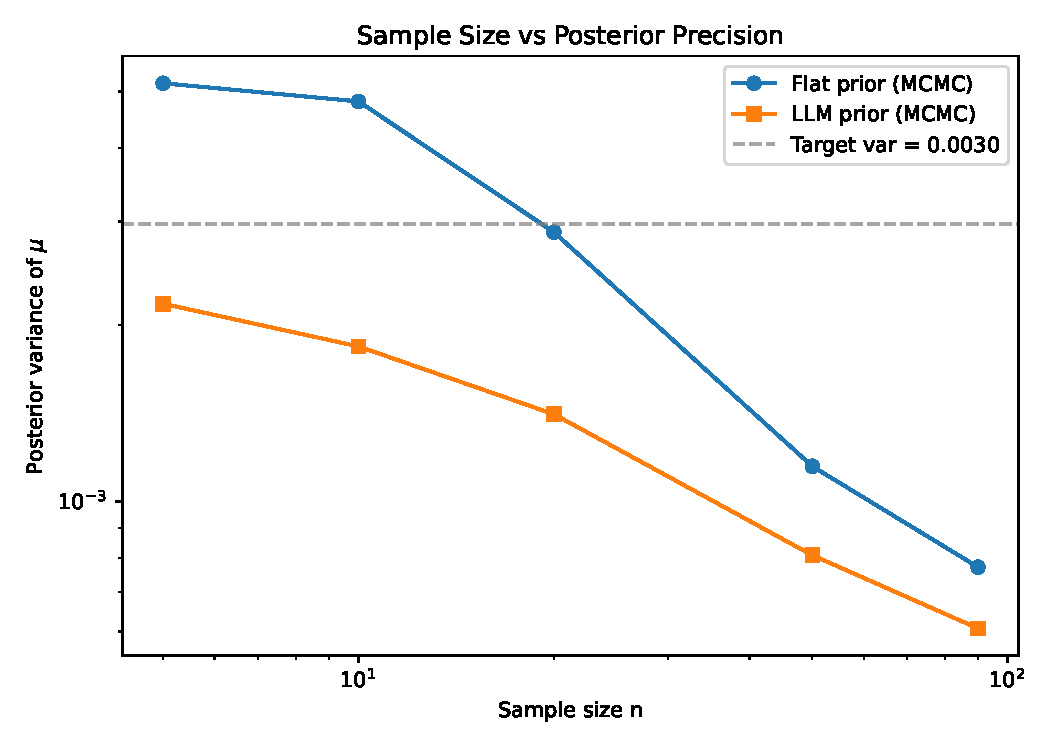
\includegraphics[width=0.65\textwidth]{../figures/nstar_curve.pdf}
  \caption{Posterior variance of $\mu$ vs.\ sample size $n$ for flat and LLM priors. The LLM prior crosses the target precision threshold at $n \approx 5$, while the flat prior requires $n \approx 19$.}
  \label{fig:nstar}
\end{figure}

%%% ============================================================
\section{Preliminary Failure Mode Analysis}
%%% ============================================================

We test robustness to prior misspecification by artificially shifting the LLM pseudo-observations by $\delta \in \{-2, -1, 0, +1, +2\}$ standard deviations and measuring empirical coverage of 95\% posterior predictive intervals on the held-out test set ($n_{\mathrm{test}} = 41$).

\begin{table}[h]
  \centering
  \small
  \begin{tabular}{rccc}
    \toprule
    Prior shift $\delta$ & Pseudo-obs mean & Coverage & Nominal \\
    \midrule
    $-2$ & $\approx 0.10$ & 0.976 & 0.95 \\
    $-1$ & $\approx 0.20$ & 0.976 & 0.95 \\
    $0$ (original) & 0.299 & 0.976 & 0.95 \\
    $+1$ & $\approx 0.53$ & \textbf{0.829} & 0.95 \\
    $+2$ & $\approx 0.76$ & 0.976 & 0.95 \\
    \bottomrule
  \end{tabular}
  \caption{Coverage under prior misspecification. Upward shift of $+1$ std degrades coverage to 83\%.}
  \label{tab:failure}
\end{table}

\textbf{Key finding:} The LLM prior is most harmful when moderately misspecified in the upward direction ($\delta = +1$, prior mean $\approx 0.53$ vs.\ data mean $0.36$).
Extreme misspecification ($|\delta| = 2$) is less harmful because the data overwhelms the prior.
This asymmetry reflects the fact that GPT-4o's unshifted prior ($\bar{y} = 0.299$) lies slightly below the human data mean, so upward shifts move it further from truth while downward shifts or extreme shifts are neutralized by the data.

%%% ============================================================
\section{Evaluation Plan \& Remaining Work}
%%% ============================================================

\paragraph{Completed.}
\begin{itemize}
  \item Data preparation (137 dictator game observations, train/test split)
  \item LLM prior elicitation (500 GPT-4o pseudo-observations)
  \item Baseline: flat prior + MCMC (Metropolis--Hastings)
  \item Frontier: LLM prior + SVGD (Stein Variational Gradient Descent)
  \item Sample size reduction ratio $\rho = 0.26$
  \item Preliminary failure mode analysis (prior misspecification)
\end{itemize}

\paragraph{Remaining for final report (due April 27).}
\begin{enumerate}
  \item \textbf{Extended calibration:} Coverage analysis at multiple significance levels and sample sizes; calibration plots (expected vs.\ observed coverage).
  \item \textbf{Compute--accuracy tradeoff:} Wall-clock time comparison and effective sample size for SVGD vs.\ MCMC at matched posterior precision.
  \item \textbf{Game variant comparison:} Run the full pipeline on the ``taking game'' variant (68 observations) to test whether the LLM prior generalizes across framing conditions.
  \item \textbf{Finer failure mode analysis:} Denser shift grid ($\delta \in [-3, +3]$ in steps of 0.5); coverage vs.\ prior weight $w$ sensitivity.
  \item \textbf{Reproducibility:} Fixed seeds, \texttt{environment.yml}, README with exact reproduction commands.
\end{enumerate}

\paragraph{Code repository.}
All code is available at: \url{https://github.gatech.edu/bfeng66/cse8803-iuq-project} (private, collaborators \texttt{pchen402} and \texttt{psi6} added).

\vspace{1em}

\bibliography{references}

\end{document}
